\documentclass[11pt]{article}

\usepackage[T1]{fontenc}
\usepackage{lmodern}
\usepackage{amsmath,amssymb,amsthm}
\usepackage{graphicx}
\usepackage{xcolor}
\usepackage[margin=1in]{geometry}
\usepackage{hyperref}
\hypersetup{
  colorlinks=true,
  linkcolor=blue!50!black,
  citecolor=blue!50!black,
  urlcolor=blue!50!black
}

\newtheorem{theorem}{Theorem}[section]
\newtheorem{proposition}[theorem]{Proposition}
\newtheorem{lemma}[theorem]{Lemma}
\newtheorem{corollary}[theorem]{Corollary}
\theoremstyle{definition}
\newtheorem{definition}[theorem]{Definition}
\theoremstyle{remark}
\newtheorem{remark}[theorem]{Remark}

\newcommand{\C}{\mathbb C}
\newcommand{\R}{\mathbb R}
\newcommand{\eps}{\varepsilon}
\newcommand{\dd}{\mathrm d}
\newcommand{\Dfinite}{D\text{-finite}}
\newcommand{\NE}{NE}
\newcommand{\Ht}{H}
\newcommand{\Jt}{J}

\title{Non-\texorpdfstring{$D$}{D}-finiteness of irreducible
\texorpdfstring{$NE$}{NE}-prudent ramps}
\author{Self-Avoiding Walk Lab}
\date{12 September 2026}

\begin{document}

\maketitle

\begin{center}
\fbox{\parbox{0.91\textwidth}{\small
\textbf{Publication candidate; priority unresolved; not externally peer
reviewed.}  The theorem below is presented as an internally reviewed
mathematical draft.  The statement concerns the irreducible
\(NE\)-prudent-ramp series \(J\) only.  It makes no claim about the
weakly prudent bridge quotient \(W\), the square-lattice connective constant,
or publication priority.}}
\end{center}

\begin{abstract}
Let \(P(t)\) be the generating function for \(NE\)-prudent ramps and let
\(H(t)\) be the hook-ramp function in the explicit algebraic formulas of
Bacher and Beaton.  Their irreducible \(NE\)-prudent-ramp series is
\[
  J(t)=\frac{P(t)-H(t)}{1+P(t)}.
\]
We prove that \(J\) is not \(D\)-finite.  The proof starts from the exact
kernel expressions and their meromorphic continuation.  A change of
parameter \(q=U(t,1)=\exp(-\varepsilon/2)\) isolates a critical crossing in
the iterated product defining \(P\) and \(H\).  The product is factored
exactly into a smooth factor and a Gamma ratio.  Uniform Gamma estimates,
an integrable bound at the crossing, and exponential control of the far tail
give uniform limits for two regularized moments.  Their limits are four
one-dimensional integrals with an explicit singular profile.  Outward
dyadic interval arithmetic certifies endpoint signs for the limiting
functions and a positive hook margin throughout a phase interval.  For all
sufficiently large integer indices, continuity then gives a zero of
\(1+P\) with \(1+H>0\).  These zeros yield infinitely many non-removable
poles of \(J\), which is impossible for a \(D\)-finite analytic germ.
\end{abstract}

\noindent\textbf{Keywords:} self-avoiding walks; prudent walks; generating
functions; \(D\)-finite series; kernel method; Gamma products.

\section{Introduction}

Prudent self-avoiding walks are walks on the square lattice that never step
towards a previously visited vertex.  They form several nested subclasses
whose generating functions exhibit a range of behaviours between directed
models and unrestricted self-avoiding walks.  We use the following precise
convention.  A walk \(\omega=(\omega_0,\ldots,\omega_n)\) is rooted at the
origin, and its bounding box is the smallest axis-parallel rectangle
containing its vertices.  A walk is prudent when no step points towards a
previously visited vertex, and it is \(NE\)-prudent when it is prudent and,
for every prefix, the prefix endpoint lies on the north or east side of that
prefix's bounding box.  It is a bridge when, writing \(y_i=y(\omega_i)\),
 \(y_0<y_i\leq y_n\) for every \(i\geq1\).  A bridge is a ramp when
\(x(\omega_i)\leq x(\omega_n)\) for every \(0\leq i\leq n\); throughout,
ramps are nonempty bridges.  Bridge
concatenation is the usual concatenation at the endpoint; ``irreducible''
means that no factorization into two shorter bridges exists.  All generating
functions below weight a walk by \(t^{n}\), with no quotient by lattice
symmetries.

In the model studied here, Bacher and Beaton introduced weakly prudent
bridges and expressed the irreducible \(NE\)-prudent-ramp series in terms of
two auxiliary functions.  Their Theorem~17 gives the meromorphic
continuation and the infinitely many source poles accumulating at
\(\sigma=\sqrt2-1\) \cite{BacherBeaton2014}; see also the
\href{https://dmtcs.episciences.org/2445/pdf}{official PDF}.  The quotient
defining the irreducible series requires a separate noncancellation argument.

We use the notation
\[
  J(t)=\frac{P(t)-H(t)}{1+P(t)}.
\]
Here \(P\) counts the \(NE\)-prudent ramps and \(H\) is the hook-ramp
function denoted \(\widetilde P\) in the source.  The common poles of \(P\)
and \(H\) do not by themselves survive in this quotient: at a common simple
pole the local principal parts can cancel after the quotient is formed.
Our argument instead finds infinitely many zeros of \(1+P\) between
successive source poles and proves that the numerator \(-1-H\) is nonzero
at those zeros.

\begin{theorem}[Main result]\label{thm:main}
The formal power series at the origin represented by
\[
  J(t)=\frac{P(t)-H(t)}{1+P(t)}
\]
is not \(D\)-finite.
\end{theorem}

The proof is conditional only on the exact formulas and meromorphic
continuation theorem established in \cite{BacherBeaton2014}; all additional
limits and signs needed for the quotient are proved below.  The interval
calculation used to evaluate the limiting integrals is described explicitly,
including its endpoint substitutions and outward rounding.  It does not use
floating-point quadrature error as a proof.

Our conclusion is deliberately narrow.  We do not transfer it to the
additional weakly prudent bridge series \(W\), do not state a formula for any
square-lattice connective constant, and do not make a claim of being first.

\IfFileExists{figures/critical_phase.pdf}{%
\begin{figure}[t]
  \centering
  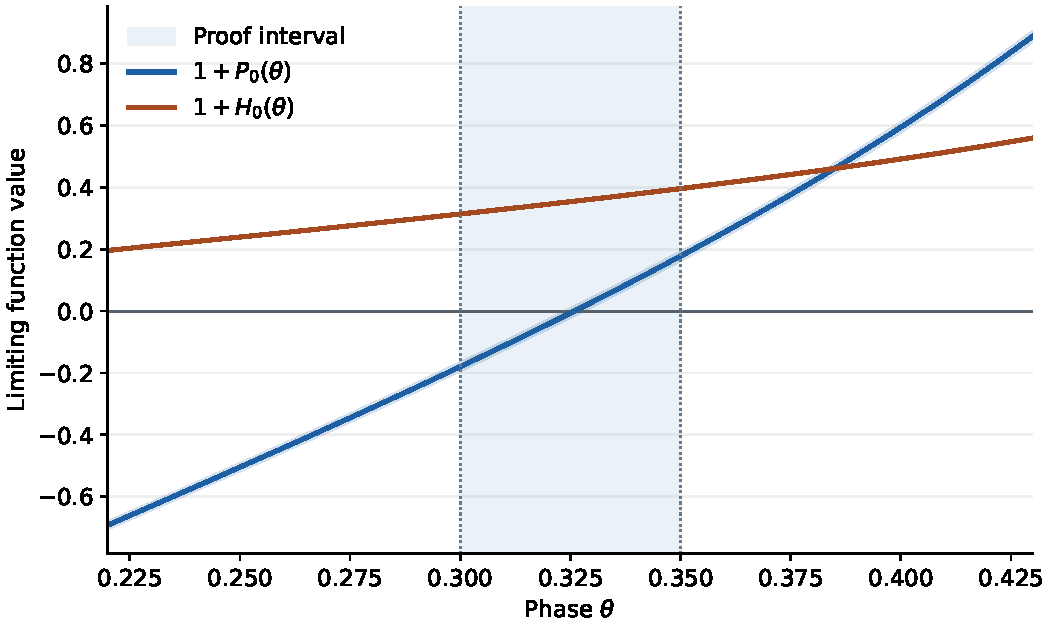
\includegraphics[width=0.88\textwidth]{figures/critical_phase.pdf}
  \caption{Illustrative limiting phase plot for \(1+P_0\) and \(1+H_0\).
  The shaded interval is \(\theta\in[0.30,0.35]\), and the bands visualize
  the certified integral coefficient intervals; the exact sign conclusions
  are the interval statements in Section~\ref{sec:certificate}.}
  \label{fig:critical-phase}
\end{figure}
}{}

\section{The exact Bacher--Beaton functions}\label{sec:source}

We first record the formulas used in the proof.  This fixes the branch,
normalization, and all auxiliary quantities before any limiting operation.
For \(t\) and \(v\) near the origin, set
\[
  \alpha(t,v)=1-tv+t^2+t^3v
\]
and let
\begin{equation}\label{eq:kernel}
  U(t,v)=
  \frac{\alpha(t,v)-\sqrt{\alpha(t,v)^2-4t^2}}{2t}.
\end{equation}
The square root is the branch for which \(U(t,v)=t+O(t^2)\).  Put
\[
  q=U(t,1),\qquad
  u_n=U(t,q^{2n}),\qquad
  w_n=U(t,q^{2n+2}).
\]
For the real parameter range used later, all of these quantities are on the
same physical branch.

Write
\[
  C=q-t,\qquad D=1-tq,\qquad E=1-q^2,
  \qquad h(u)=tq-Cu.
\]
For \(u,w\) on the physical branch, define
\begin{align}
 {\cal A}(t;u,w)
  &=
  \frac{C(1-t^2)
   \bigl(Du-[qC+tEu]w\bigr)}
  {D(1-tu)(1-tw)h(u)},                                      \label{eq:A}\\
 {\cal B}(t;u,w)
  &=
  \frac{qC^2\bigl(t-Dw\bigr)}
  {D^2h(u)},                                                 \label{eq:B}\\
 \widetilde{\cal A}(t;u,w)
  &=
  \frac{t^2(1-t^2)C}
  {D(1-tu)^2(1-tw)^2h(u)}
  \nonumber\\
  &\quad{}\times
  \bigl[
    Du^2(1-2tw)
    -\{qC-tu(2qC+tEu)\}w^2
  \bigr].                                                    \label{eq:Ah}
\end{align}
Let \(p_0=1\) and
\[
  p_{n+1}=p_n{\cal B}(t;u_n,w_n).
\]
Then the two functions from Propositions 14 and 16 of
\cite{BacherBeaton2014} are
\begin{align}
 P(t)
   &=\frac{q(1-t^2)}{D}
     +q\sum_{n\geq0}p_n{\cal A}(t;u_n,w_n),                  \label{eq:P}\\
 H(t)
   &=\frac{t^2q^2(1-t^2)}{D^2}
     +q\sum_{n\geq0}p_n\widetilde{\cal A}(t;u_n,w_n).        \label{eq:H}
\end{align}
For fixed \(t\) away from the source poles, these sums converge in the
meromorphic continuation supplied by the source.  The series at the origin
is the germ to which the continuation is attached.

The kernel equation at \(v=1\) gives
\begin{equation}\label{eq:q-relation}
  q+\frac1q=\frac1t-1+t+t^2.
\end{equation}
At \(t=\sigma=\sqrt2-1\), the right side equals \(2\), and its derivative
with respect to \(t\) is nonzero.  Thus the smaller branch \(q<1\) can be
used as a local parameter near \(\sigma\).

The source proves in Theorem~17 that \(P\) and \(H\) have simple real poles
\(a_0<a_1<\cdots<\sigma\), with \(a_\ell\to\sigma\), and no other poles
between consecutive members of this sequence.  In the notation above,

\begin{equation}\label{eq:source-poles}
 h(u_n)=0
 \quad\Longleftrightarrow\quad
 (q-t)(u_n-t)=t^2
 \quad\Longleftrightarrow\quad
 \frac{(q-t)(U(t,q^{2n})-t)}{t^2}=1.
\end{equation}

Thus the zeros of the displayed denominator are exactly the pole
characterization used in that theorem.  We use this continuation theorem to
evaluate the formulas on the intervals constructed below.

\section{Exact algebra and regularized moments}\label{sec:algebra}

The critical argument is easier after a common algebraic reduction of the
two summands.  Define
\[
  g(u)=t-Du,\qquad
  f(u)=\frac{u}{1-tu},\qquad
  k=\frac{qC^2}{D^2}.
\]
Two identities following from \eqref{eq:q-relation} are
\begin{equation}\label{eq:CD}
  CD=tq(1-t^2),
  \qquad
  h(u)-kg(u)=\frac{CE}{D}(1-u).
\end{equation}
For \(p\geq0\), put
\[
  {\cal A}_p(t;u,w)
   =\frac{C(1-t^2)}{Dh(u)}
     \bigl(Df(u)^p-qC f(w)^p\bigr).
\]
Direct expansion of \eqref{eq:A} and \eqref{eq:Ah} gives
\begin{equation}\label{eq:Ap}
  {\cal A}={\cal A}_1,
  \qquad
  \widetilde{\cal A}=t^2{\cal A}_2.
\end{equation}
For example,
\[
 Df(u)-qCf(w)
 =\frac{Du-[qC+tEu]w}{(1-tu)(1-tw)},
\]
which proves the first equality.  For the hook term, the numerator identity
\[
\begin{aligned}
 Df(u)^2-qCf(w)^2
={}&
 \frac{Du^2(1-2tw)}{(1-tu)^2(1-tw)^2}\\
&-
 \frac{\{qC-tu(2qC+tEu)\}w^2}
 {(1-tu)^2(1-tw)^2}
\end{aligned}
\]
proves the second.

Let
\[
  g_n=g(u_n),\qquad h_n=h(u_n),\qquad z_n=\frac{p_n}{g_n}.
\]
The product recurrence becomes
\begin{equation}\label{eq:zrec}
  z_{n+1}
   =z_n\,\frac{qC}{D}\,
     \frac{g_n}{g_n+\delta},
  \qquad
  \delta=\frac{t^2E}{C}.
\end{equation}
The following telescoping identity is exact:
\begin{equation}\label{eq:tel}
\begin{aligned}
 p_n{\cal A}_p(t;u_n,w_n)
  ={}&Y_{p,n}-Y_{p,n+1}\\
   &-t^2E(1-t^2)\frac{p_nf(u_n)^p}{h_ng_n},
\end{aligned}
\end{equation}
where
\[
  Y_{p,n}=p_n\,\frac{D(1-t^2)f(u_n)^p}{g_n}.
\]
Indeed, substitution of \eqref{eq:Ap} into the right side reduces
\eqref{eq:tel} to \(Dh(u)-t^2E=Cg(u)\), which is equivalent to
\eqref{eq:CD}.  The fixed-\(t\) tail is locally geometric, so summing
\eqref{eq:tel} gives the two exact moment representations
\begin{align}
 P(t)&=\frac{C}{g(q)}
       +\sum_{n\geq0}W_nf(u_n),                              \label{eq:momentP}\\
 H(t)&=t^2f(q)\frac{C}{g(q)}
       +t^2\sum_{n\geq0}W_nf(u_n)^2,                         \label{eq:momentH}
\end{align}
where
\begin{equation}\label{eq:W}
  W_n=-qt^2E(1-t^2)\frac{p_n}{h_ng_n}.
\end{equation}
The same algebra gives the exact zeroth-moment relation
\begin{equation}\label{eq:zeromoment}
  \sum_{n\geq0}W_n(1-u_n)=-\frac{tD^2}{g(q)}.
\end{equation}
This relation is signed; it is not a positivity estimate.

The summands in \eqref{eq:momentP}--\eqref{eq:momentH} have apparent poles at
the zeros of \(h\).  We remove them before taking the critical limit.  Let
\[
  u_h=\frac{tq}{C},\qquad h(u_h)=0,
  \qquad
  L_j=\frac{f(u_h)^j}{1-u_h},
\]
and
\[
  R_j(u)=f(u)^j-L_j(1-u),\qquad j=1,2.
\]
Since \(h(u)=-C(u-u_h)\),
\begin{equation}\label{eq:regularization}
 -\frac{R_j(u)}{h(u)}
 =
 \frac{1}{C}\left[
   \frac{f(u)^j-f(u_h)^j}{u-u_h}+L_j
 \right],
\end{equation}
with the diagonal value interpreted by continuity.  The right side is
uniformly bounded on the physical interval for \(t\) near \(\sigma\).
Writing
\[
  Q=qt^2E(1-t^2),\qquad S_0=-\frac{tD^2}{g(q)},
\]
the exact regularized moments are
\begin{align}
 P(t)
  &=\frac{C}{g(q)}+L_1S_0
    -Q\sum_{n\geq0}z_n\frac{R_1(u_n)}{h_n},                  \label{eq:regP}\\
 \frac{H(t)}{t^2}
  &=f(q)\frac{C}{g(q)}+L_2S_0
    -Q\sum_{n\geq0}z_n\frac{R_2(u_n)}{h_n}.                  \label{eq:regH}
\end{align}
The cancellation in \eqref{eq:regularization} is exact at finite \(t\);
no divergent moments are subtracted only after taking a limit.

\section{Critical parameter and phase}\label{sec:phase}

Set
\[
  \eps=-\log(q^2),\qquad q=e^{-\eps/2}.
\]
Equation \eqref{eq:q-relation} and the implicit function theorem give a real
analytic function \(t=t(\eps)\) near \(\eps=0\), with
\[
  t(0)=\sigma,\qquad t(\eps)<\sigma\quad(\eps>0\text{ small}).
\]
For \(s\geq0\), define
\[
  g_\eps(s)=t-DU(t,e^{-s}).
\]
The function \(g_\eps\) has a simple positive zero \(s_g(\eps)\).  The zero
of \(g_\eps(s)+\delta\) is denoted by \(s_h(\eps)\).  At the critical point,
\[
  s_g(\eps)\longrightarrow s_*=
  -\log\left(\frac12+\frac{\sqrt2}{4}\right),
  \qquad
  U(\sigma,e^{-s_*})=u_*=\frac1{\sqrt2}.
\]
The local algebraic kernel has no branch singularity at this positive
crossing.  Differentiating the kernel relation at the crossing gives
\[
  \frac{s_g-s_h}{\eps}\longrightarrow
  \eta=\frac1{\sqrt2},
  \qquad
  \frac{-\log(qC/D)}{\eps}\longrightarrow
  \lambda=\frac1{1-\sigma}.
\]
In particular, \(\eta<1\), the fact that will make the crossing integrable.

Define
\[
  a=\frac{s_g}{\eps},\qquad b=\frac{s_h}{\eps}.
\]
Then \(b=a-\eta_\eps\), where \(\eta_\eps=\eta+O(\eps)\).  Fix the compact
phase interval
\[
  {\cal T}=\left[\frac3{10},\frac7{20}\right].
\]
Since \(s_g(\eps)=s_*+O(\eps)\), one has
\[
  \frac{\dd a}{\dd\eps}=-\frac{s_*}{\eps^2}+O(1).
\]
Therefore, for every sufficiently large integer \(N\) and every
\(\theta\in{\cal T}\), there is a unique small \(\eps_N(\theta)\) such that
\begin{equation}\label{eq:phase}
  a(\eps_N(\theta))=N+\theta.
\end{equation}
The inverse is continuous in \(\theta\), and
\(\eps_N(\theta)=s_*/N+O(N^{-2})\) uniformly on \({\cal T}\).  The
separation of \({\cal T}\) from the integers, together with
\(\eta=1/\sqrt2\), implies that \(a\) and \(b\) remain a fixed positive
distance from all integers.  Thus no \(g_\eps(n\eps)\) or
\(g_\eps(n\eps)+\delta\) vanishes in the phase family.

\section{Matched Gamma products}\label{sec:gamma}

The product in \eqref{eq:zrec} is singular near the crossing, so it must not
be replaced there by an Euler approximation.  We factor its singular part
exactly.  For a fixed \(S>s_*+1\), set
\[
 F_\eps(s)=\frac{g_\eps(s)}{s-s_g},\qquad
 G_\eps(s)=\frac{g_\eps(s)+\delta}{s-s_h},\qquad
 R_\eps(s)=\frac{F_\eps(s)}{G_\eps(s)}.
\]
The removable values at the two zeros are filled in by the corresponding
positive derivatives.  At \(s_j=j\eps\),
\[
 \frac{g_\eps(s_j)}{g_\eps(s_j)+\delta}
 =
 \frac{j-a}{j-b}R_\eps(s_j).
\]
Consequently, with \(r=qC/D\),
\begin{equation}\label{eq:gamma-factor}
 z_n=z_0r^nT_n(a,b)
      \prod_{j=0}^{n-1}R_\eps(j\eps),
\qquad
 T_n(a,b)=\prod_{j=0}^{n-1}\frac{j-a}{j-b}.
\end{equation}
The singular product has the exact Gamma representation
\begin{equation}\label{eq:Tgamma}
  T_n(a,b)=
  \frac{\Gamma(n-a)\Gamma(-b)}
       {\Gamma(-a)\Gamma(n-b)}.
\end{equation}
All products at \(n=0\) are one.

The smooth factor has a uniform limit.  On \(0\leq s\leq S\),
\[
  \frac{\log R_\eps(s)}{\eps}
  \longrightarrow
  \psi(s)=-\frac{\kappa}{g_0(s)}
            +\frac{\eta}{s-s_*},
\qquad
  \kappa=\frac{\sigma^2}{1-\sigma},
\]
where the apparent pole at \(s_*\) is removable.  To prove this, take a
fixed neighborhood of \(s_*\).  There \(g_\eps\) is analytic with a uniformly
simple zero, and Taylor expansion in the two root locations gives the
uniform first-order expansion of the ratio of divided differences.  Outside
that neighborhood,
\[
 \log R_\eps(s)=
 \log\left(1+\frac{s_g-s_h}{s-s_g}\right)
 -\log\left(1+\frac{\delta}{g_\eps(s)}\right),
\]
and both terms have uniformly bounded denominators and are \(O(\eps)\).
The explicit square-root expression \eqref{eq:kernel} gives uniform
convergence of \(g_\eps\) on the whole compact interval, including \(s=0\).
The two local descriptions agree at \(s_*\), so the Riemann-sum limit is
uniform:
\begin{equation}\label{eq:Rsump}
 \sum_{j<n}\log R_\eps(j\eps)
 \longrightarrow \int_0^s\psi(x)\,\dd x,
 \qquad n\eps\longrightarrow s.
\end{equation}
Likewise \(n\log r\to-\lambda s\), uniformly on bounded \(s\)-intervals.

For the Gamma factor, use the reflection formula and the uniform
parameter version of the Gamma-ratio asymptotic
\(\Gamma(x+c)/\Gamma(x+d)\sim x^{c-d}\).  These are the standard identities
\cite[Eq.~5.5.3]{DLMF55} and \cite[Eq.~5.11.12]{DLMF511}; the exact
source pages are
\href{https://dlmf.nist.gov/5.5.E3}{DLMF 5.5.3} and
\href{https://dlmf.nist.gov/5.11.E12}{DLMF 5.11.12}.  If
\(n\eps\to s\) and \(s\ne s_*\), then
\begin{equation}\label{eq:Tlimit}
 T_n(a,b)\longrightarrow
 \begin{cases}
 \displaystyle
  \left(\frac{s_*}{|s-s_*|}\right)^\eta,
     &s<s_*,\\[1.2ex]
 \displaystyle
  \frac{\sin(\pi\theta)}{\sin(\pi(\theta-\eta))}
  \left(\frac{s_*}{|s-s_*|}\right)^\eta,
     &s>s_*.
 \end{cases}
\end{equation}
The rate \(\eta_\eps-\eta=O(\eps)\) is essential: it implies
\((\eta_\eps-\eta)\log\eps\to0\), so no unnoticed power of \(\eps\) remains.
The convergence is uniform on compact \(s\)-subintervals avoiding \(s_*\)
and uniformly in \(\theta\in{\cal T}\).

We also need a bound through the crossing.  For \(n\leq N\), reflection is
not needed and the positive-argument identity is
\[
 T_n=
 \frac{\Gamma(a+1)\Gamma(b-n+1)}
      {\Gamma(b+1)\Gamma(a-n+1)}.
\]
For \(n\geq N+1\), reflection gives
\[
 T_n=
 \frac{\sin(\pi a)}{\sin(\pi b)}
 \frac{\Gamma(a+1)\Gamma(n-a)}
      {\Gamma(b+1)\Gamma(n-b)}.
\]
All Gamma arguments that can be small remain a fixed distance from zero
because of the phase restrictions.  Uniform positive-argument Gamma-ratio
bounds therefore give, for any fixed \(\nu>0\) with
\(\eta+\nu<1\),
\begin{equation}\label{eq:localbound}
 |z_n|\leq C_S
 \bigl(\eps+|n\eps-s_g|\bigr)^{-\eta-\nu},
 \qquad n\eps\leq S,
\end{equation}
with \(C_S\) independent of \(N\) and \(\theta\).  The smooth product and
\(r^n\) are bounded on this compact scale.  Beyond a fixed
\(S>s_*+1\), \(g_\eps\) is uniformly positive and
\[
  0<\frac{g_\eps(s)}{g_\eps(s)+\delta}\leq1,
  \qquad
  r\leq e^{-c\eps}
\]
for some \(c>0\).  The recurrence then gives
\begin{equation}\label{eq:tailbound}
 |z_n|\leq C e^{-c(n\eps-S)},\qquad n\eps\geq S.
\end{equation}
The first index beyond \(S\) is controlled by \eqref{eq:localbound}.  This
proves the uniform product and tail bounds required below.

\section{The limiting product profile}\label{sec:profile}

At criticality write
\[
  u=U(\sigma,e^{-s}),\qquad d=1-\sigma,\qquad
  u_*=\frac1{\sqrt2}.
\]
The inverse relation between \(s\) and \(u\) is
\begin{equation}\label{eq:phi}
  e^{-s}=\phi(u)
  =\frac{(u-\sigma)(1-\sigma u)}
         {\sigma(1-\sigma^2)u}.
\end{equation}
The limiting logarithmic derivative obtained from
\eqref{eq:Rsump}, \eqref{eq:Tlimit}, and \(n\log r\) is
\begin{equation}\label{eq:profile-ode}
 \frac{\dd}{\dd s}\log|Z(u(s))|
 =-\lambda-\frac{\kappa}{g_0(s)}.
\end{equation}
Substitution of \eqref{eq:phi} into the right-hand side and elementary
partial fractions verify the explicit profile below on each side of \(u_*\).
Normalize the positive profile by
\[
\begin{aligned}
 M_{\rm raw}(u)
  &=(u-\sigma)^{2+\sqrt2}
    \left(\frac1\sigma-u\right)^{\sqrt2}
    |u-u_*|^{-\eta}u^{-1-\sqrt2},\\
 M(u)&=\frac{M_{\rm raw}(u)}{M_{\rm raw}(1)}.
\end{aligned}
\]
Let
\[
  A_*=\frac1{\sigma^2},\qquad
  B(\theta)=A_*
   \frac{\sin(\pi\theta)}{\sin(\pi(\eta-\theta))}.
\]
For \(\theta\in{\cal T}\), \(B(\theta)>0\).  Combining
\eqref{eq:gamma-factor}, \eqref{eq:Rsump}, and \eqref{eq:Tlimit}, while
using \(g_0(0)=-\sigma^2\), gives the two-sided limiting product
\begin{equation}\label{eq:profile}
 Z_\theta(u)=
 \begin{cases}
  -A_*M(u),&u_*<u\leq1,\\
  B(\theta)M(u),&\sigma<u<u_*.
 \end{cases}
\end{equation}
The relative amplitude in the second line is not a free choice: it is the
reflection multiplier in \eqref{eq:Tlimit}.  This is the connection
information that would be lost by solving only the formal differential
equation for the smooth product.

\section{Uniform convergence of the regularized moments}\label{sec:moments}

At the critical point let
\[
  f(u)=\frac{u}{1-\sigma u},\qquad
  L=2+\sqrt2,\qquad
  K=\sigma^2(1-\sigma^2).
\]
The limits of the finite-\(\eps\) regularizers in
\eqref{eq:regularization} are
\[
\begin{aligned}
 V_1(u)
  &=\frac1d\left[
       L+\frac1{u_*(1-\sigma u)}
     \right],\\
 V_2(u)
  &=\frac1d\left[
       L+\frac{f(u)+1}{u_*(1-\sigma u)}
     \right].
\end{aligned}
\]
Both are continuous and positive on \([\sigma,1]\).  The boundary terms in
\eqref{eq:regP}--\eqref{eq:regH} have the limits \(-d\) and \(-3\),
respectively, after the factor \(t^2\) is removed from the second equation.
This follows by substituting \(t\to\sigma\), \(q\to1\), and
\eqref{eq:CD}; also \(Q/\eps\to K\).

Define four finite positive integrals:
\begin{align}
 J_{j,\mathrm{pre}}
  &=K\int_{u_*}^{1}
     M(u)V_j(u)\frac{\phi'(u)}{\phi(u)}\,\dd u,              \label{eq:Jpre}\\
 J_{j,\mathrm{post}}
  &=K\int_{\sigma}^{u_*}
     M(u)V_j(u)\frac{\phi'(u)}{\phi(u)}\,\dd u,
 \qquad j=1,2.                                              \label{eq:Jpost}
\end{align}
The only interior singularity is
\(|u-u_*|^{-\eta}\), with \(\eta<1\), so both integrals converge.
Uniformly for \(\theta\in{\cal T}\), the regularized moment sums converge to
\begin{align}
 P_0(\theta)
  &=-d-A_*J_{1,\mathrm{pre}}
     +B(\theta)J_{1,\mathrm{post}},                         \label{eq:P0}\\
 H_0(\theta)
  &=\sigma^2\left[
       -3-A_*J_{2,\mathrm{pre}}
       +B(\theta)J_{2,\mathrm{post}}
     \right].                                                \label{eq:H0}
\end{align}

\begin{proof}[Proof of the uniform moment convergence]
Fix a small \(\nu>0\) with \(\eta+\nu<1\), and a crossing window
\(|n\eps-s_g|<\rho\).  The divided-difference formula
\eqref{eq:regularization} gives a uniform bound for the regularized factor
\(R_j(u_n)/h_n\).  Hence \eqref{eq:localbound} bounds the absolute
contribution of the crossing window by
\[
 C\eps\sum_{|n\eps-s_g|<\rho}
 \bigl(\eps+|n\eps-s_g|\bigr)^{-\eta-\nu}
 \leq C'(\rho+\eps)^{1-\eta-\nu}.
\]
This tends to zero uniformly when first \(\eps\to0\) and then
\(\rho\to0\).  There is no residual point mass at the crossing.

Outside this window, the product convergence
\eqref{eq:Rsump} and \eqref{eq:Tlimit} are uniform, so ordinary Riemann-sum
convergence gives \eqref{eq:Jpre}--\eqref{eq:H0}.  The endpoint \(s=0\)
is covered by \eqref{eq:localbound}; the square-root behaviour of the
algebraic kernel there is not differentiated in the argument.  Finally,
\eqref{eq:tailbound} gives a uniform exponentially small bound beyond the
fixed \(S\).  Letting \(S\to\infty\) completes the proof uniformly in
\(\theta\).
\end{proof}

\section{Certified signs of the limiting functions}\label{sec:certificate}

We now describe the exact sign certificate for \eqref{eq:P0} and
\eqref{eq:H0}.  It is included to distinguish a rigorous interval
calculation from a floating-point quadrature.

For the pre-integrals in \eqref{eq:Jpre}, substitute
\[
  u=u_*+(1-u_*)x^8,\qquad 0\leq x\leq1.
\]
For the post-integrals, use
\[
  u=u_*-(u_*-\sigma)x^8,\qquad 0\leq x\leq1,
\]
with the orientation reversed so that the integral runs from \(\sigma\) to
\(u_*\).  In both cases
\[
  |u-u_*|^{-\eta}|\,\dd u\,|
  =8\Delta^{1-\eta}x^{8(1-\eta)-1}\,\dd x,
\]
where \(\Delta\) is the corresponding interval length.  The exponent
\(8(1-\eta)-1\) is strictly positive.

The certificate partitions \([0,1]\) into 2048 equal bins.  It encloses
every nonnegative base and exponent by dyadic intervals, evaluates
sixteenth-bit exponent bounds using 16 outward square roots and integer
powers, and takes the hull when a base interval straddles one.  Endpoint
factors are algebraically cancelled before interval evaluation.  The
constant \(\pi\) is enclosed with Machin's identity and alternating
arctangent remainders; the sine factor in \(B(\theta)\) is enclosed by a
Taylor polynomial with its Lagrange remainder.  All arithmetic in this
calculation is rational outward interval arithmetic.

The resulting decimal displays of the certified integral intervals are
\[
\begin{array}{c|cc}
 &J_1&J_2\\ \hline
\mathrm{pre}
 &[0.45986641,\,0.46232754]&[0.650478,\,0.65423355]\\
\mathrm{post}
 &[0.42401814,\,0.42637240]&[0.56790451,\,0.57100730].
\end{array}
\]
Substitution into the limiting functions gives
\[
\begin{array}{c|cc}
\theta&1+P_0(\theta)&1+H_0(\theta)\\ \hline
3/10
 &[-0.19278831,\,-0.16685274]
 &[0.31077599,\,0.31715257]\\
7/20
 &[0.16373676,\,0.19165184]
 &[0.39270347,\,0.39952767].
\end{array}
\]
The displayed intervals are rounded outward from the exact dyadic
enclosures.

The hook margin holds throughout the phase interval, not only at its
endpoints.  Indeed,
\[
 B'(\theta)=
 A_*\frac{\pi\sin(\pi\eta)}
 {\sin^2(\pi(\eta-\theta))}>0
\]
on \({\cal T}\), and \(J_{2,\mathrm{post}}>0\).  Thus \(H_0(\theta)+1\)
is increasing, and
\begin{equation}\label{eq:Hmargin}
  H_0(\theta)+1>0.310
  \qquad(\theta\in{\cal T}).
\end{equation}

\section{Infinitely many non-removable poles}\label{sec:conclusion}

We now prove the main theorem.  For each sufficiently large \(N\), define
\[
  t_N(\theta)=t(\eps_N(\theta)),
  \qquad\theta\in{\cal T},
\]
using \eqref{eq:phase}.  Uniform convergence in
\eqref{eq:P0}--\eqref{eq:H0} and the strict certified margins imply
\[
  P(t_N(3/10))<-1
  <P(t_N(7/20)),
  \qquad
  H(t_N(\theta))+1>0
  \quad(\theta\in{\cal T})
\]
for all sufficiently large \(N\).  The source pole sequence is avoided
throughout these phase intervals by the distance conditions on \(a\) and
\(b\), so \(P\) and \(H\) are analytic there.  Continuity gives a point
\(r_N\) in the interval with
\[
  P(r_N)=-1.
\]
At this point,
\[
  P(r_N)-H(r_N)=-1-H(r_N)\ne0.
\]
Consequently \(J\) has a non-removable pole at \(r_N\).  The intervals for
different \(N\) are disjoint because their phase parameters satisfy
\(a=N+\theta\), and \(r_N\to\sigma\).  We have therefore produced infinitely
many distinct finite-plane poles of the analytic continuation of \(J\).

For completeness, recall the elementary \(D\)-finite obstruction.  If a
nonzero analytic germ at the origin is \(D\)-finite, then it satisfies a
linear differential equation with polynomial coefficients.  Its analytic
continuation can have finite singularities only at zeros of the leading
coefficient of that equation, a finite set.  The infinitely many poles just
constructed contradict this property.  Theorem~\ref{thm:main} follows.
\qed

\section{Scope and reproducibility}\label{sec:scope}

The exact starting formulas \eqref{eq:P}--\eqref{eq:H}, the algebraic
identities, the product factorization, the uniform bounds, and the limiting
integral signs are separate proof components.  The interval certificate
described in Section~\ref{sec:certificate} is a finite exact-arithmetic
certificate for the displayed limiting integrals; the passage from the
discrete products to those integrals is supplied by
Sections~\ref{sec:gamma}--\ref{sec:moments}.

The proof establishes non-\(D\)-finiteness only for \(J\).  It does not
establish the corresponding claim for the weakly prudent bridge quotient
\(W\), and it does not assert an exact growth constant for unrestricted
self-avoiding walks.  The priority of the result is unresolved and the
draft has not been externally peer reviewed.

\bibliographystyle{plain}
\bibliography{references}

\end{document}
